%\documentclass[12pt]{article}
\documentclass[BCOR=12mm,DIV11,titlepage,a4paper,oneside]{scrbook}
\usepackage{scrhack}
\usepackage[ngerman]{babel}
\usepackage[utf8x]{inputenc}
\usepackage{amsmath}
\usepackage{graphicx}
\usepackage{caption}
\usepackage[colorinlistoftodos]{todonotes}
\usepackage{subcaption}

%fancyheadings funktioniert nicht mehr mit der KOMA Script Klasse scrbook

\usepackage{wrapfig}

\usepackage[authoryear,round]{natbib}

% Mittels [H] können Bilder genau an einer Stelle positioniert werden
\usepackage{float}

\usepackage[breaklinks]{hyperref}

% bewirkt das HyperLinks in der PDF nicht umrandet oder farbig sind
\hypersetup{colorlinks=false}

% package for colored text
% black,white,green,red,blue,yellow,cyan,magenta
\usepackage{color}

% package for colored tables
\usepackage{colortbl}

%Paket zur Erzeugung von Anführungszeichen durch \enquote{Text}
\usepackage[ngerman]{babel}
\usepackage[babel, german=quotes]{csquotes}

%Verhindern, dass eine neue Seite für ein einzelnes Wort/Zeile verwendet wird
\clubpenalty = 10000 % schliesst Schusterjungen aus 
\widowpenalty = 10000 % schliesst Hurenkinder aus (keine Beleidigung, sondern wirklich ein Fachbegriff)

\usepackage{lipsum}

\begin{document}

%!TEX root = ../main.tex
\begin{titlepage}

\begin{center}

% Logo der Technische Hochschule Köln
% Kann auch in dieser Form in Schwarz/Weiß ausgedruckt werden; Graustufen sollten der .tif Version entsprechen
\begin{figure}[!ht]
%	\centering
		
\includegraphics[width=0.26\textwidth]{images/THlogoheader.pdf}
\end{figure}

\vspace{0.4cm}

%Deutscher Titel
\begin{rmfamily}
\begin{huge}
\textbf{Titel}\\	
\end{huge}
\vspace{0.5cm}
\begin{LARGE}
mit einem eventuell\\ganz langen Untertitel\\
\end{LARGE}
\end{rmfamily}

\vspace{0.8cm}

%Englischer Titel
% \begin{rmfamily}
% \textbf{\LARGE Title in English}\\
% \large with a very\\long subtitle\\
% \normalsize
% \end{rmfamily}

% \vspace{1.2cm}

%Bachelorarbeit 
\begin{LARGE}
\begin{scshape}
Bachelorarbeit\\[0.8em]
\end{scshape}
\end{LARGE}

%ausgearbeitet von...
\begin{large}
ausgearbeitet von\\ 
\vspace{0.3cm}
\begin{LARGE}
Max Mustermann\\
\end{LARGE}
\end{large}

\vspace{1.2cm}

%zur Erlangung des akademischen Grades...
\begin{large}
zur Erlangung des akademischen Grades\\
\vspace{0.1cm}
\textsc{Bachelor of Science (B.Sc.)}\\ 
\end{large}

\vspace{0.6cm}

%vorgelegt an der...
\begin{large}
vorgelegt an der\\ 
\vspace{0.2cm}
\begin{scshape}
Technischen Hochschule Köln\\
Campus Gummersbach\\
Fakultät für Informatik und\\
Ingenieurwissenschaften\\
\end{scshape}
\end{large}

\vspace{0.6cm}

%im Studiengang...
\begin{large}
im Studiengang\\ 
\vspace{0.1cm}
\textsc{Medieninformatik}
\end{large}


\vspace{1.2cm}

%Autor der Bachelorarbeit und die Prüfer
\begin{tabular}{rl}
        Erster Prüfer/in:  &  Prof. Dr. Peter Silie\\
       					&  \small Technische Hochschule Köln \\[1.0em]
       Zweiter Prüfer/in:  &  Prof. Dr. Maria Musterprof\\
       					&  \small Technische Hochschule Köln\\
\end{tabular}

\vspace{1.2cm}

%Ort, Monat der Abgabe
\begin{large}
Gummersbach, im August \the\year
\end{large}

\end{center}

\newpage
\thispagestyle{empty}

%Kontaktmöglichkeiten des Autors und der Prüfer
\begin{center}
\begin{tabular}{rl}
							&  \\[26.0em]
							
\large \textbf{Adressen:}	&  	\quad Max Mustermann\\
							&  	\quad Musterstraße 1\\
							&	\quad 12345 Musterstadt\\
							&  	\quad max@mustermann.de\\[2.0em]
							
							&  	\quad Prof. Dr. Peter Silie\\
							&  	\quad Technische Hochschule Köln\\
							&  	\quad Institut für Informatik\\
							&	\quad Steinmüllerallee 1\\
							&	\quad 51643 Gummersbach\\
							&  	\quad peter.silie@th-koeln.de\\[2.0em]
							
							&  	\quad Prof. Dr. Maria Musterprof\\
							&  	\quad Technische Hochschule Köln\\
							&  	\quad Institut für Informatik\\
							&	\quad Steinmüllerallee 1\\
							&	\quad 51643 Gummersbach\\
							&  	\quad maria.musterprof@th-koeln.de\\[2.0em]
\end{tabular}
\end{center}

\end{titlepage}


\tableofcontents
\setcounter{page}{1}
\newpage

\chapter*{Kurzfassung}
Fügen Sie hier die Kurzfassung Ihrer Arbeit, welche bestenfalls strukturiert sein sollte, z.B. Einleitung, Hintergrund, Problemstellung, Zielsetzung, Vorgehen/Methode, Ergebnis, Fazit. 

Hier ein recht bekanntes Beispiel für Abstracts von \textit{Nature}-Artikel:
\url{http://unl.libguides.com/c.php?g=51569&p=2633458}

\newpage
\chapter*{Abstract}
Hier folgt die Kurzfassung auf Englisch. Wenn Sie diese Vorlage für Seminararbeiten, Projektdokumentation o.ä. verwenden ist eine englische Kurzfassung ggf. nicht nötig.

\newpage
\chapter{Einleitung}
\label{cha:Einleitung}

In diesem Dokument werden einige Beispiele gegeben, die Ihnen das Erstellen Ihrer Arbeit erleichtern soll. Wir geben Ihnen hier Tipps zum Umgang mit \LaTeX, aber auch einige Hinweise zum Erstellen wissenschaftlicher Arbeiten. 

Wenn Sie ein neues Kapitel beginnen, beachten Sie bitte, dass dieses ebenfalls eine Einleitung aufweist. Das heißt, dass Kapitelüberschriften \textit{nicht} für sich alleine stehen und beispielsweise direkt die Überschrift des ersten Abschnittes folgt.


\section{Tabellen}
\label{sec:Tabellen}
Dieser Abschnitt gibt Beispiele für die Verwendung von Tabellen.

\begin{table}[ht]
	\centering
    \caption[Kurztitel Tabelle]{Hier steht der lange Titel für die Tabelle}
    \vspace{1.0em}	
	\begin{tabular}{|l|r|}
\hline
Text & 12\% \\
\hline
Text & 34\% \\
\hline
Text & 56\% \\
\hline
Text & 78\% \\
\hline
Text & 90\% \\
\hline
		\end{tabular}
	\vspace{1.0em}
	\label{tab:tabelle}
\end{table}

\noindent{}Dies ist lediglich ein Beispiel. Je nach beabsichtigter Aussage, können Tabellen ganz unterschiedlich aussehen. Ein weiteres Beispiel:

\begin{table}[ht]
	\centering
	\caption[Alternative Tabelle]{Alternative Tabelle mit farbiger Kopfzeile}
		\vspace{1.0em}	
	\begin{tabular}{|c|l|}
		\hline
		\rowcolor[gray]{0.9}\textbf{numbers} & \textbf{text} \\
		\hline
		\hline
		1 & This text flush-left \\
		\hline
		2 & while the numbers are \\
		\hline
		3 & centred \\
		\hline
	\end{tabular}
	\label{tab:tablealternative}
\end{table}

Bitte beachten Sie: Tabellen haben in der Regel \textit{Über}schriften, während Abbildungen \textit{Unter}schriften aufweisen. Im Quellcode sehen Sie, dass im "caption" ein kurzer Titel vergeben wird, der für das Tabellenverzeichnis vergeben wird. Der längere Titel wird als Überschrift verwendet.  \\

Das Erstellen von Tabellen kann sehr aufwändig sein. Die folgenden Werkzeuge können hier sehr hilfreich sein:

\begin{itemize}
	\item Excel to \LaTeX{} Converter\\ \url{https://github.com/krlmlr/Excel2LaTeX/releases}
	\item Apple Script: Numbers to \LaTeX{} \\ \url{https://gist.github.com/pgundlach/386384}
	\item Gnumeric (hat eine Export-Funktion für \LaTeX{}): \\ \url{https://projects.gnome.org/gnumeric/}
	\item OpenOffice, Calc2LaTeX: \url{http://extensions.openoffice.org/de/project/calc2latex-macro-converting-openofficeorg-calc-spreadsheets-latex-tables}
\end{itemize}

\section{Tabellen referenzieren}
\label{sec:tabellen_ref}
In diesem Abschnitt werden die Tabellen aus dem vorigen Abschnitt im Text referenziert. Dies ist der Bezug auf die erst Tabelle: \ref{tab:tabelle}, und hier der Verweis auf die zweite Tabelle \ref{tab:tablealternative}. Vergeben Sie am besten immer jeder Tabelle, Abbildung, Abschnitt, Kapitel, etc. ein individuelles label, so dass Sie dieses dann zum Referenzieren verwenden können. Im Übrigen stehen Abbildungen und Tabellen niemals für sich alleine, sondern sollten im Text diskutiert werden und somit natürlich auch referenziert. Die Verwendung des "ref{}"-Befehls sorgt dafür, dass immer auf die richtige Nummerierung verwiesen wird, selbst wenn der Text später geändert wird (z.B., wenn Tabellen hinzugefügt oder gelöscht werden). 

\section{Anführungszeichen}
\label{sec:Anfuehrungszeichen}

Es gibt verschiedene Optionen, Anführungszeichen zu generieren. Da das entsprechende Paket eingebunden wurde, können Sie folgende Optionen verwenden:

\begin{itemize}
	\item \enquote{Befehl des Pakets: csquotes}
	\item Alternativ: ``example''
	\item Oder "Beispiel". 
\end{itemize}

Wie Ihnen vielleicht aufgefallen ist, sehen die Alternative etwas anders aus. Für die Verwendung von Anführungszeichen gibt es Konventionen, siehe \url{https://de.wikibooks.org/wiki/LaTeX-W%C3%B6rterbuch:_Anf%C3%BChrungszeichen}






\newpage
%!TEX root = ../VorlageBA.tex
\chapter{Kapitel Zwei}
Hier würde eine Einleitung zum Kapitel stehen... 

\section{Abbildungen in LaTeX}
\label{sec:abbildungen_in_latex}

Beispiel für eine Grafik:
\begin{figure}[!ht]
	\centering
		%[natürliche Breite in Pixeln, natürliche Höhe in Pixeln, Abhängigkeit von der Textbreite]
		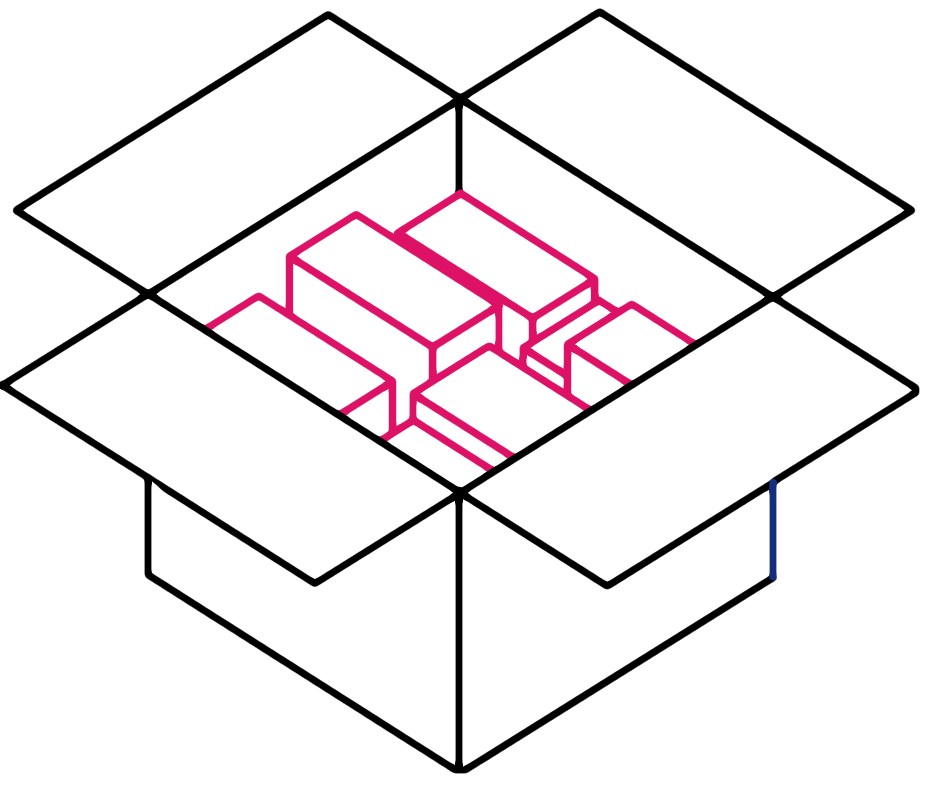
\includegraphics[width=0.75\textwidth]{images/MIBox.png}
	\caption{Bildunterschrift mit einer Quelle \citep{Autor2013}}
	\label{fig:box}
\end{figure}

Eine Abbildung sollte immer im Text diskutiert werden und dann entsprechend mit dem \texttt{ref{}}-Befehl referenziert werden. Bitte beachten Sie auch, dass die Quelle entsprechend angegeben wird. An dieser Stelle wurde exemplarisch mit dem \texttt{cite{}} Befehl ein Quelle hinzugefügt.

\section{Zitierweise}
Dies ist ein Beispiel für ein wörtliches Zitat:
\begin{quotation}
	\emph{``A persona is a rich picture of an imaginary person who represents your core user group.''} \citep{Dix04}
\end{quotation}

Alternativ könnte man auch schreiben: 
\begin{quotation}
	\textit{\enquote{A persona is a rich picture of an imaginary person who represents your core user group.}} \citep{Dix04}
\end{quotation}

Das Ergebnis im Dokument ist hier gleich. \\

Manchmal möchte man die Autorennamen im Text verwenden. Bislang haben wir den \texttt{citep\{\}} Befehl verwendet. Hierdurch werden die Klammern um Autorname und Jahr gesetzt. Man kann den \texttt{cite} Befehl allerdings auch variieren: \\

\cite{Dix04} definieren das Konzept "Persona" wie folgt: 
\begin{quotation}
	\emph{``A persona is a rich picture of an imaginary person who represents your core user group.''}
	\citep{Dix04}
\end{quotation}

Das richtige Setzen der Klammern erhöht die Lesbarkeit. \\

Im APA Format\footnote{ American Psychological Association (APA)} gibt es einige Regeln, wann und wie man Seitenzahlen bei den Literaturverweisen verwendet:

\begin{quotation}
	\emph{``Include page numbers for any citations in the text of your paper that include direct quotations or refer to a specific part of the work you are referencing. Direct quotations must include a page number as part of the citation. The quoted material should be followed by a citation in parentheses that gives the author's name, the year in which the work was published, and the page number from which the quoted material appears.''}
	\citep{Hall}
\end{quotation}

Weitere Beispiele und Empfehlungen von \cite{Hall} finden Sie hier:  \url{http://www.ehow.com/how_5689799_cite-numbers-apa-format.html}. In \LaTeX{} kann man die Seitenzahlen sehr einfach hinzufügen, zum Beispiel: \\

\citet[S. 86]{Baddeley:1974ts} führen aus: 

\begin{quotation}
	\emph{``We hope that our preliminary attempts to begin answering the question will convince the reader, not necessarily that our views are correct, but that the question was and is well worth asking''}
	\citep[p. 86]{Baddeley:1974ts}
\end{quotation}

Im ersten Verweis auf \citeauthor{Baddeley:1974ts} haben wir \texttt{citet[]\{\}} verwendet, um die Klammern um das Jahr zu setzen. Im zweiten Fall im Anschluss an das Zitat wurde \texttt{citep[]\{\}} verwendet.

\section{Verweise innerhalb des Dokumentes} % (fold)
\label{sec:verweise_im_dokument}

Wenn Sie auf Ihre eigenen Kapitel, Abbildungen, Tabellen o.ä. verweisen wollen, können Sie den \texttt{ref\{\}} Befehl verwenden, wie auch bereits vorab gezeigt im Abschnitt~\ref{sec:tabellen_ref} auf Seite~\pageref{sec:tabellen_ref}.  \\

An dieser Stelle möchten wir nun auf die MI Box verweisen. Sie hat die Abbildungsnummer~\ref{fig:box} und ist auf Seite \pageref{fig:box} zu finden. Wie Sie an diesem Beispiel auf dieser Seite sehen, kann man mit \LaTeX{} nicht nur auf die Abschnitts-/ oder Tabellennummer verweisen, sondern auch auf die Seitenzahl auf der das Label verweist. Wenn Sie diese dynamischen Codes verwenden (statt zum Beispiel die Nummerierung manuell einzutragen), haben Sie immer die korrekte Nummerierung, auch wenn Sie den Text später umstrukturieren. Wir nutzen den \texttt{pageref\{\}} Befehl hierfür.

% section verweise_im_dokument (end)




\newpage
\chapter{Weitere Kapitel}
\label{cha:weitere_kapitel}

\section{Fußnoten und Listen} % (fold)
\label{sec:fussnoten_listen}
Fußnoten können zum Teil sehr nützlich sein. Bitte beachten Sie, dass bei übermäßiger Verwendung von Fußnoten, die Lesbarkeit einschränkt sein kann\footnote{ da der Lesefluss unterbrochen wird!}. 

\subsection{Beispiel Unterabschnitte} % (fold)
\label{sub:bsp_unterabschnitt}
Sie können in \LaTeX{} Unterabschnitte verwenden. Wenn Sie allerdings einen Unterabschnitt einfügen, sollten es mindestesns zwei sein. Es ist unüblich, dass man beispielsweise nur einen Abschnitt in einem Kapitel hat, oder nur einen Unterabschnitt in einem Abschnitt. Siehe zum Beispiel folgenden Tipp von Dave Patterson: 

\begin{quotation}
	\emph{``Its strange to have a single subsection (e.g., 5.2.1 in section 5.2). Why do you need to number it if there is only one? Either eliminate the single subsection, or change the part that precedes the subsection into a second subsection''}
	\citep{Patterson2013}
\end{quotation} 

% subsection bsp_unterabschnitt (end)


\subsection{Listen} % (fold)
\label{sub:listen}
Hier folgen einige Beispiele für Listen. Zunächst eine nicht nummerierte Liste: 

\begin{itemize}
	\item Item 1
	\item Item 2
	\item Item 3
\end{itemize}

Nun eine nummerierte Liste:

\begin{enumerate}
	\item Item 1
	\item Item 2
	\item Item 3
\end{enumerate}

Man kann auch Symbole verwenden:

\begin{itemize}
\renewcommand{\labelitemi}{$\rightarrow$}
	\item Item 1
	\item Item 2
	\item Item 3
\end{itemize}

\subsubsection{Beispiel für Unter-Unterabschnitt} % (fold)
\label{ssub:bsp_unterunterabschnitt}
Die gängige Gliederungstiefe von 3 Ebenen (Kapitel, Abschnitt, Unterabschnitt) sollte in der Regel nicht unterschritten werden. Sie können zwar eine weitere Ebene tiefer gehen, da dies ggf. die Lesbarkeit verringert wird diese in \LaTeX{} nicht automatisch im Inhaltsverzeichnis aufgeführt. Hier werden beispielhaft Unter-Unterabschnitte verwendet. 

Der folgende Text ist lediglich ein Platzhalter: \emph{Lorem ipsum dolor sit amet, consetetur sadipscing elitr, sed diam nonumy eirmod tempor invidunt ut labore et dolore magna aliquyam erat, sed diam voluptua. At vero eos et accusam et justo duo dolores et ea rebum. Stet clita kasd gubergren, no sea takimata sanctus est Lorem ipsum dolor sit amet.}

% subsubsection bsp_unterunterabschnitt (end)

\subsubsection{Noch ein Unter-Unterabschnitt}
Der folgende Text ist lediglich ein Platzhalter, welchen man auch automatisch mit dem Paket ``Lipsum'' generieren kann: 
\textit{\lipsum[1]}	

\paragraph{Paragraph als Alternative} % (fold)
\label{par:paragraph_als_alternative}
Für diesen Abschnitt wurde nicht der \texttt{subsubsection\{\}} Befehl verwendet, sondern ``paragraph'', der auch verwendet werden kann, um einen Unterabschnitt zu generieren. Verglichen zum \texttt{subsubsection\{\}} Befehl beginnt der Text hier nicht in einer neuen Zeile, sondern direkt nach der Überschrift. Wenn Ihr Dokument eher kurz gehalten ist, kann dies kann eher angemessen sein.
% paragraph paragraph_als_alternative (end)

% subsection listen (end)

% section fussnoten_listen (end)

\section{description-Umgebung} % (fold)
\label{sec:description_umgebung}
Wenn Sie bestimmte Konzepte beschreiben wollen, ist eine Liste oder ein Unterabschnitt ggf. nicht der beste Weg. Als Alternative gibt es außerdem die \emph{description} Umgebung, die hier nützlich sein kann.

\begin{description}
	\item[Konzept A] Lorem ipsum dolor sit amet, consetetur sadipscing elitr, sed diam nonumy eirmod tempor invidunt ut labore et dolore magna aliquyam erat, sed diam voluptua. At vero eos et accusam et justo duo dolores et ea rebum. Stet clita kasd gubergren, no sea takimata sanctus est Lorem ipsum dolor sit amet.
	\item[Konzept B] Lorem ipsum dolor sit amet, consetetur sadipscing elitr, sed diam nonumy eirmod tempor invidunt ut labore et dolore magna aliquyam erat, sed diam voluptua.
\end{description}

% section description_umgebung (end)

% chapter additional_chapter (end)



\newpage
%Erzeugt ein Abbildungsverzeichnis
	\listoffigures
	%Fügt die Zeile "`Abbildungsverzeichnis"' als Chapter ins Inhaltsverzeichnis ein
	\addcontentsline{toc}{chapter}{Abbildungsverzeichnis}
\newpage
	
	%Erzeugt ein Tabellenverzeichnis
	\listoftables
	%Fügt die Zeile "`Tabellenverzeichnis"' als Chapter ins Inhaltsverzeichnis ein
	\addcontentsline{toc}{chapter}{Tabellenverzeichnis}
\newpage

% To change the title from References to Bibliography:
\renewcommand\refname{Literaturverzeichnis}

%Paket für ein deutsches Literaturverzeichnis

\bibliographystyle{natdin} % or try natplain or unsrtnat
\bibliography{literatur} % refers to literatur.bib

	%Fügt die Zeile "`Literaturverzeichnis"' als Chapter ins Inhaltsverzeichnis ein
	\addcontentsline{toc}{chapter}{Literaturverzeichnis}
\newpage

%!TEX root = ../Masterthesis_Fischer.tex
\chapter*{Eidesstattliche Erklärung}
%\addcontentsline{toc}{chapter}{Eidesstattliche Erklärung}

Ich versichere, die von mir vorgelegte Arbeit selbständig verfasst zu haben.\\ \\
Alle Stellen, die wörtlich oder sinngemäß aus veröffentlichten oder nicht veröffentlichten Arbeiten anderer entnommen sind, habe ich als entnommen kenntlich gemacht. Sämtliche Quellen und Hilfsmittel, die ich für die Arbeit benutzt habe, sind angegeben.\\ \\
Die Arbeit hat mit gleichem Inhalt bzw. in wesentlichen Teilen noch keiner anderen Prüfungsbehörde vorgelegen.
\vspace{1.5cm}
\\
Gummersbach, \today
\vspace{3cm}
\\
Max Mustermann


% chapter eidesstattliche_erklärung (end)

\end{document}